All above-mentioned sequencing techniques are aimed to investigate only one cellular compartment at a time, but in order to obtain a more comprehensive view of the cellular behaviour, it is necessary to look at more than one omics at the same time.

\begin{figure}[H]
\centering
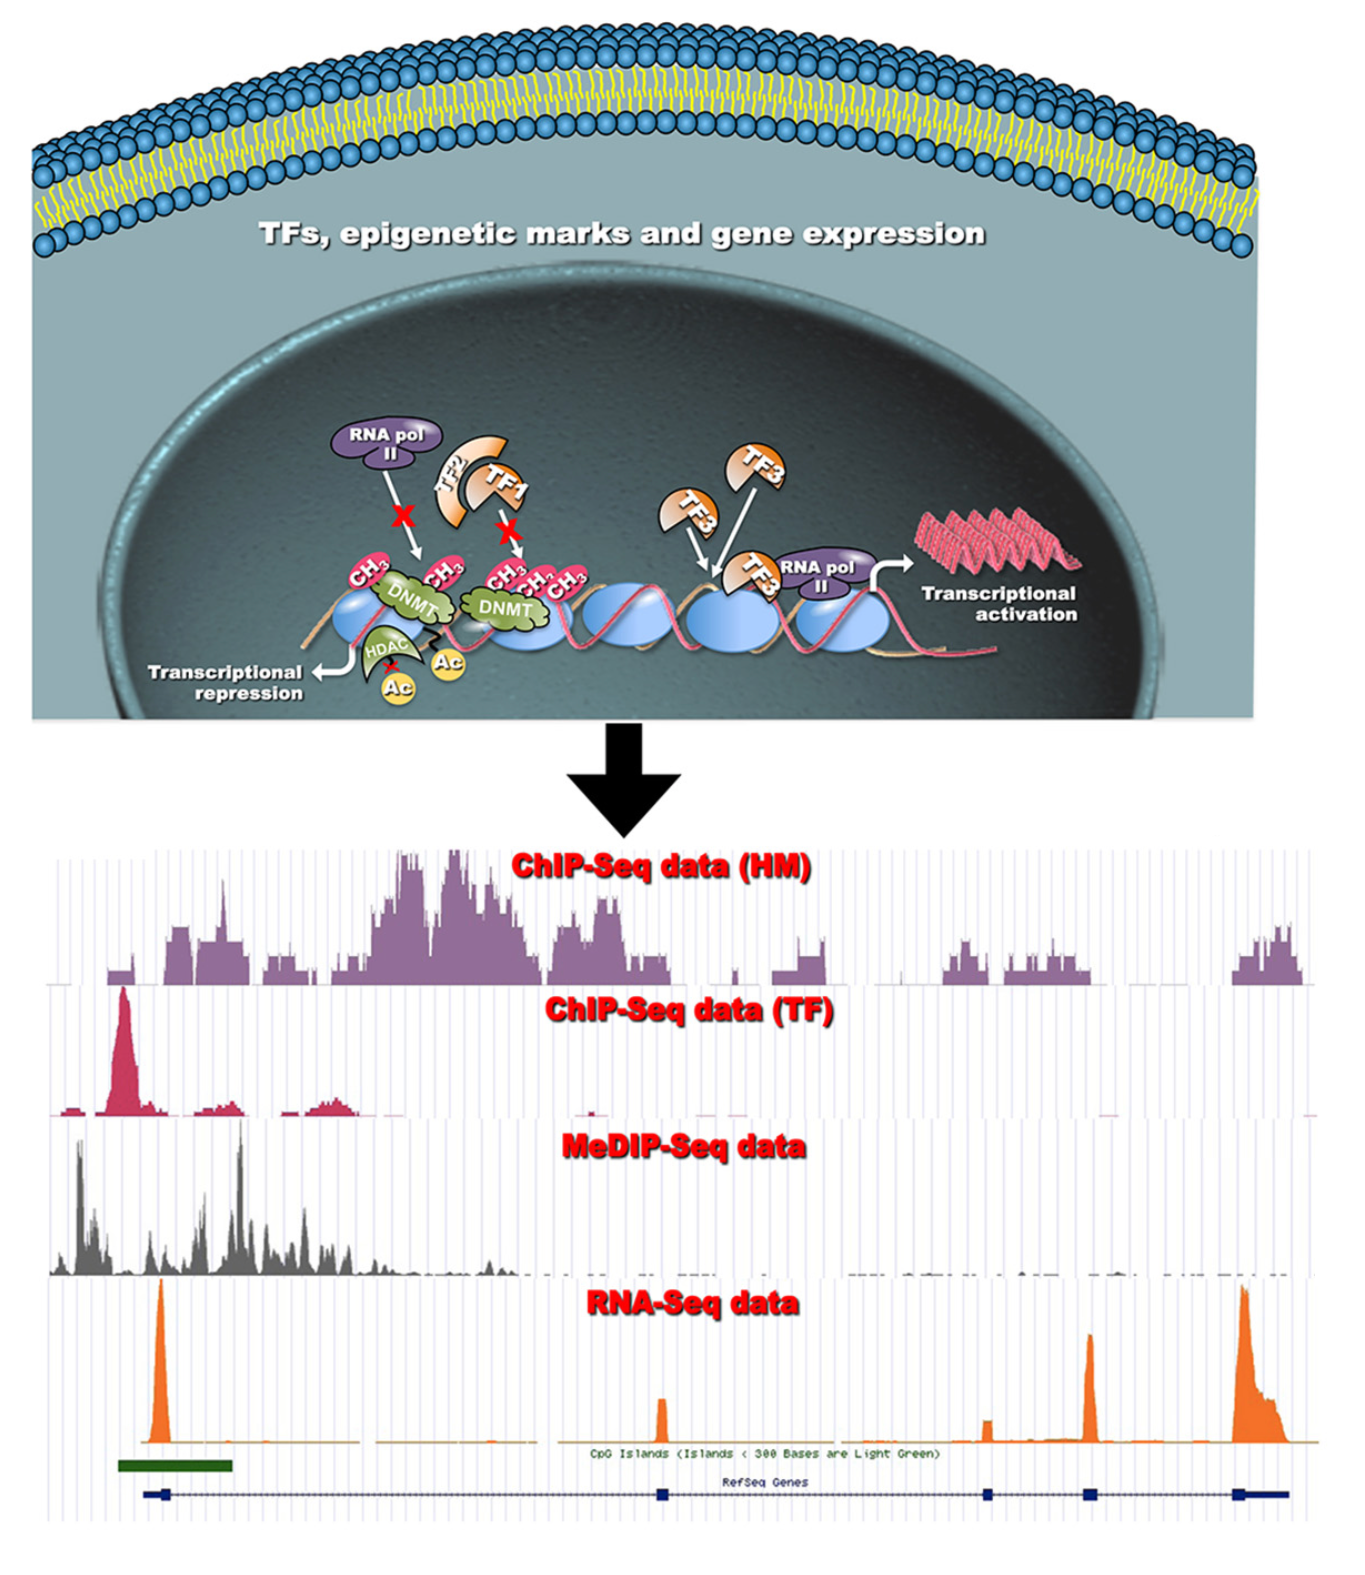
\includegraphics[width=9cm, keepaspectratio]{img/intro/multiomicsex.png}
\caption[Multi-Omics Representation]{An example of different omics coming from the same biological experimental conditions. 
An \glspl{hm} (such as \textit{Acetylation}) can have inhibited the accession to bind specific nucleosomes, because already occupied by specific \glspl{tf}, inhibiting, in such a way, the expression of those genes present in that particular portion of the chromatin (upper part).
To investigate these processes, we can perform multiple experiments of \gls{rnaseq} and \gls{chipseq} (one for the \gls{hm} and one for the \gls{tf}) to study singularly each epigenomics factors and the gene expression (lower part) \cite{Angelini2014c}.}
\label{fig:omics}
\end{figure}

Indeed, we can imagine each omics as a camera in a multi-view camera system pointed on a building from different points of view.
Each device takes snapshots of the building from different angles, but the information is still fragmented.
In order to reconstruct a 3D model of the building, we need to put all the snapshots coming from different devices together.

\begin{figure}[h]
\centering
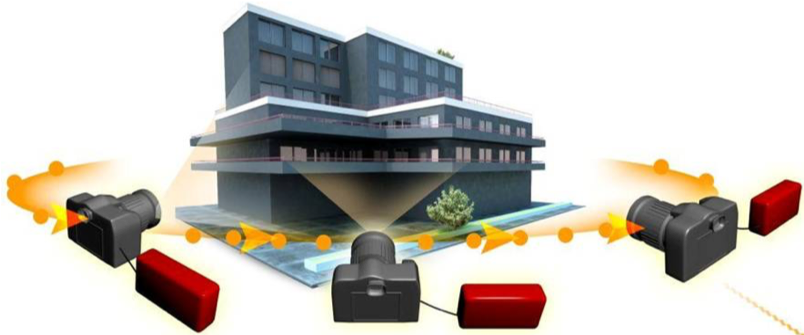
\includegraphics[width=8cm, keepaspectratio]{img/intro/cameras.png}
\caption[Integration cameras]{An illustrative exaple of a multi-view camera system pointed on a building.
Each omics can be represented by a different camera pointed on the same building. 
The final snapshots can be integrated to reconstruct the building, which represents the cellular behaviour.}
\label{fig:cameras}
\end{figure}

The same idea can be adapted to the sequencing techniques, we need to integrate the information coming from different omics in order to reconstruct (and understand) how multiple mechanisms orchestrate the cellular behaviour.

Indeed, we can imagine a typical combination of epigenomics factors affecting the chromatin in order to influence the transcription of one or more genes.
An \gls{hm} (such as \textit{Acetylation}) can have inhibited the accession to bind specific nucleosomes, because already occupied by specific \glspl{tf}, inhibiting, in such a way, the expression of those genes present in that particular portion of the chromatin (upper part of figure \ref{fig:omics}).
To investigate these processes, we can perform multiple experiments of \gls{rnaseq} and \gls{chipseq} (one for the \gls{hm} and one for the \gls{tf}) to study singularly each epigenomic factors and the gene expression (lower part of figure \ref{fig:omics}). 

As figure \ref{fig:funnell} outlines, multi-omics data integration can be made at different levels, by graphical exploration, by functional annotation, by network fusion and by dimensionality reduction.
We can distinguish two main approaches; ''analyze each omics then integrate the results'' and ''jointly analyze each omics to improve the power''.
The first one can be done also with few samples, where each omics is analyzed standalone and then the results can be combined to obtain a common response (levels 1 and 2 of figure \ref{fig:funnell}).
The second main approach needs a high number of samples to analyze all the omics together to obtain more power in the response prediction (levels 3 and 4 of figure \ref{fig:funnell}) \cite{Rohart2017, Argelaguet2018, Jia2017, Meng2016}.

\begin{figure}[h]
\centering
\includegraphics[width=8cm, keepaspectratio]{img/intro/funnell.pdf}
\caption[Integration Funnell]{A schematic representation of multi-omic data integration levels.
Graphical exploration can be used to visualize data coming from different sources (e.g. \gls{rnaseq} and \gls{chipseq}) using specific tools designed at this scope.
Functional annotation integration combines analysis results (such as relevant lists of genes) with publicly available databases to detect functional responses.
Network fusion techniques are used when a high number of data samples is available or when having multiple-omics data types coming from the same patients.
Also dimensionality reduction techniques require several samples to be able to obtain relevant and reliable results.
}
\label{fig:funnell}
\end{figure}

More in general, integration can be performed at different levels (i.e. descriptive, exploratory, inferencial, etc.).

With graphical exploration, we can visualize data coming from different sources (e.g. \gls{rnaseq} and \gls{chipseq}) using specific tools designed at this scope, such as \textit{Genome Browser} \cite{Karolchik2011} or \gls{igv} \cite{Robinson2011, Thorvaldsdottir2013} and looking to the overlapping regions, or where expressed epigenomic markers have corrispondence with gene expression sites.

We refer to functional annotation integration when using methods combining analysis results (such as relevant lists of genes) with publicly available databases,  like the Gene Ontology\footnote{http://www.geneontology.org/} and pathway (such as \textit{KEGG}\footnote{https://www.genome.jp/kegg/} or \textit{Reactome}\footnote{https://reactome.org/}) based ones, to detect functional responses highly related to the experimental condition under investigation.

It is possible to integrate multiple omics data types by constructing multiple regulation networks, one for each analyzed omics, and then combine these networks with fusion techniques.
This integration aspect is used when a high number of data samples is available or when having multiple-omics data types coming from the same patients \cite{Wang2014}.

A deeper level of integration is achievable with dimensionality reduction techniques. 
Also in this case, several samples are needed to be able to obtain relevant and reliable results.
Generally speaking, these methods are able to start from multiple samples coming from different omics and to reduce their dimensionality, enabling to identify common cellular behavioural aspects \cite{Rohart2017, Argelaguet2018}.



